% Clase del documento
\documentclass[12pt, letterpaper]{article}

% Definicion del preambulo
% Para insertar imágenes
\usepackage{graphicx}

% Para tener referencias
\usepackage{hyperref}

% Para poner matemáticas
\usepackage{amsthm, amssymb}

% Matrices
\usepackage{amsmath}

% Para poner definiciones con color
\usepackage[most]{tcolorbox}

% Colores
\usepackage{xcolor}

% Quita sangrías/Pone saltos en párrafos
%\usepackage{parskip}

% Español
\usepackage[spanish]{babel}

% imagenes svg
\usepackage{svg}

% para insertar imágenes en una posición estricta
\usepackage{float}

% Definición personalizada de tcolorbox
\newtcolorbox{miDefinicion}[2][]{
  colback=teal!5!white,
  colframe=teal!75!black,
  coltitle=white,
  fonttitle=\bfseries,
  title=Definición: #2,
  arc=2mm,
  boxrule=0.8pt,
  enhanced,
  drop shadow,
  #1
}


% Titulo, autor y fecha
\title{\textbf{\textcolor{teal}{Denavit Hartenberg}}}
\author{Ricardo Victoria}
\date{Agosto 2027}

% Inicio del documento
\begin{document}

% Insertamos el preambulo
\maketitle

% Insertamos secciones
\section{Conceptos}
Las definiciones siguientes nos ayudarán a entender el tema. Algunas de estas se describen de forma informal, y se definen en el contexto de la robótica.

% Def Eslabón
\begin{miDefinicion}{Eslabón y Nodo}
    Un \textbf{eslabón}, \textbf{enlace} o \textbf{link} es un cuerpo sólido con al menos un punto particular llamado \textbf{nodo}, \textbf{articulación} o \textbf{joint} que soporta el montaje de otro eslabón.

    \vspace{0.4cm}

    \centering
    \includegraphics[width=0.55\textwidth]{imagenes/brazo.png}
\end{miDefinicion}

%Def Marco Referencia
\begin{miDefinicion}{Marco de Referencia}
    Un \textbf{marco de referencia} (a veces se le llama \textbf{frame}, \textbf{sistema de referencia} o \textbf{sistema de coordenadas}) es un sistema de coordenadas abstracto, cuyo origen, orientación y escala se han especificado en el espacio físico. [2]

    \vspace{0.4cm}

    \centering
    \includegraphics[width=0.45\textwidth]{imagenes/brazo-marco.png }
\end{miDefinicion}

% Def Cadena cinemática abierta simple
\begin{miDefinicion}{Cadena cinemática abierta simple}
    Una \textbf{cadena cinemática abierta simple} es una secuencia \textbf{lineal} de eslabones conectados por nodos donde un eslabón está fijo (eslabón base) y otro eslabón queda libre para moverse en el espacio (efector final). [3]

    \vspace{0.4cm}

    \centering
    \includegraphics[width=0.45\textwidth]{imagenes/brazo-cadena-cinematica.png}
\end{miDefinicion}

% Def Cadena eslabón base
\begin{miDefinicion}{Eslabón base}
    Un \textbf{eslabón base} (\textbf{eslabón inicial}, \textbf{eslabón cero}, \textbf{link cero} o \textbf{$l_0$}) es el primer eslabón de una cadena cinemática abierta simple, sólo tiene un nodo, y se fija a un soporte estático o al suelo. Tiene índice cero. \todo[inline]{[lo saqué del resumen de IA de google al buscar -eslabón base robótica-]}
\end{miDefinicion}

% Def Articulacion efector final
\begin{miDefinicion}{Efector final}
    Un \textbf{efector final} (\textbf{end-effector} u \textbf{órgano terminal}) es el último eslabón de una cadena cinemática abierta simple. Este queda libre para moverse en el espacio y suele tener una pinza o un herramienta para interactuar con el entorno. Si la cadena cinemática abierta simple tiene $n$ grados de libertad (Degrees of Freedom, DoF), es decir, tiene $n$ nodos, entonces el efector final es el eslabón con índice $n$. Si el efector final tiene una pinza con una articulación prismática, a dicha articulación no se le suele considerar como nodo de la cadena cinematica abierta simple, esto porque el objetivo de D-H es ubicar al efector final a través del marco de referencia de éste; es decir, el objetivo de D-H es ubicar el marco que se coloca sobre la articulación $n$ (para una cadena cinemática con $n$ articulaciones) respecto de cualquier otro marco de la cadena cinemática. 
\end{miDefinicion}

% Def Articulación proximal y distal
\begin{miDefinicion}{Proximal y Distal}
    Una articulación proximal es cualquiera que se encuentra más cerca del centro del cuerpo, o en robótica, más cerca del eslabón base. 

    Una articulación distal es cualquiera que se encuentra más lejos del centro del cuerpo, o en robótica, más lejos del eslabón base.

    En general, proximal significa ``más cerca del eslabón base''; distal significa ``más lejos del eslabón base''.

    Para un eslabón $i$ cualquiera, su articulación proximal es la que está más cerca del eslabón base; y su articulación distal es la que está más lejos del eslabón base. 

    Para un nodo $i$ cualquiera, su eslabón proximal es el que está más cerca del eslabón base; y su eslabón distal es el que está más lejos del eslabón base. 
\end{miDefinicion}

% Def Índices de los eslabones y de las articulaciones
\begin{miDefinicion}{Indexado de eslabones y articulaciones}
    Empezamos a contar a los eslabones y a las articulaciones en el sentido que va desde el eslabón inicial y hasta el eslabón final (de proximal a distal). 

    El primer eslabón es el eslabón base, y éste tiene el índice cero (eslabón cero, link cero, $l_0$). Y así sucesivamente con los demás eslabones. 

    Por otro lado, el primer nodo (el único nodo del eslabón base) tiene el índice uno (articulación 1, $art_1$, nodo 1). Y así sucesivamente con los demás nodos. 
\end{miDefinicion}

% Articulación revoluta
\begin{miDefinicion}{Articulación revoluta}
    Una articulación revoluta (o rotacional) es una unión mecánica en robótica que permite el giro relativo entre dos eslabones alrededor de un único eje.
\end{miDefinicion}

% Articulación prismática
\begin{miDefinicion}{Articulación prismática}
    Una articulación prismática (o junta deslizante) es una conexión mecánica en robótica y mecanismos que permite un movimiento de traslación lineal en una sola dirección a lo largo de un eje.
\end{miDefinicion}
\section{¿Qué es Denait Hartenberg?}
\textbf{Denavid Hartenberg} (D-H) es un método y convención en robótica que asigna \textbf{marcos de referencia} a \textbf{eslabones} de una \textbf{cadena cinemática abierta simple}. Además, permite hacer \textbf{transformaciones} entre \textbf{marcos de referencia}, es decir, permite ubicar a un \textbf{marco de referencia} respecto de otro. En general, D-H nos permite modelar una cadena cinemática abierta simple, como un brazo robótico.

Existen otras convenciones, hay muchas formas y orientaciones para acomodar un marco de referencia (e.g. utilizar el sistema de la mano izquierda en lugar del de la mano derecha), hay diferentes ordenes para rotar y trasladar marcos de referencia. Al profundizar en diferentes recursos externos, es importante saber que pueden utilizar una convencion diferente para no confundirnos.
\section{Asignación de marcos de referencia}
A continuación definiremos los pasos de \textbf{Denavit Hartenberg} para asignar marcos de referencia. Luego veremos un ejemplo.

\begin{miDefinicion}{Denavit Hartenberg - Asignación de marcos de referencia}
    Para un eslabón $i$ con dos nodos:
    \begin{enumerate}
        \item Alinear $z_i$ con el eje en movimiento de la articulación distal.
        \item Alinear $z_{i-1}$ con el eje en movimiento de la articulación proximal.
        \item La articulación distal tendrá índice $i+1$. La articulación proximal tendrá índice $i$.
        \item El origen $o$ del marco de referencia se coloca en la intersección entre el eje $z_{i}$ y el vector normal común a los ejes $z_{i-1}$ y $z_i$. 
        \item El eje $x$ se coloca sobre el vector normal anterior. Si son paralelos, $x_i$ va de $z_{i-1}$ a $z_i$. 
        \item El eje $y_i$ se elige con la regla de la mano derecha. 
    \end{enumerate}
\end{miDefinicion}

Ahora veremos un ejemplo utilizando el brazo robótico de la figura~\ref{fig:brazo-propio}. En este ejemplo, dibujaremos los ejes $z$ con lineas punteadas, esto significa que todos los ejes $z$ apuntan hacia nosotros, no apuntan a ninguna dirección dentro del dibujo en 2D. De hecho, en algunos recursos no se dibujan. 

\begin{figure}[H]
    \centering
    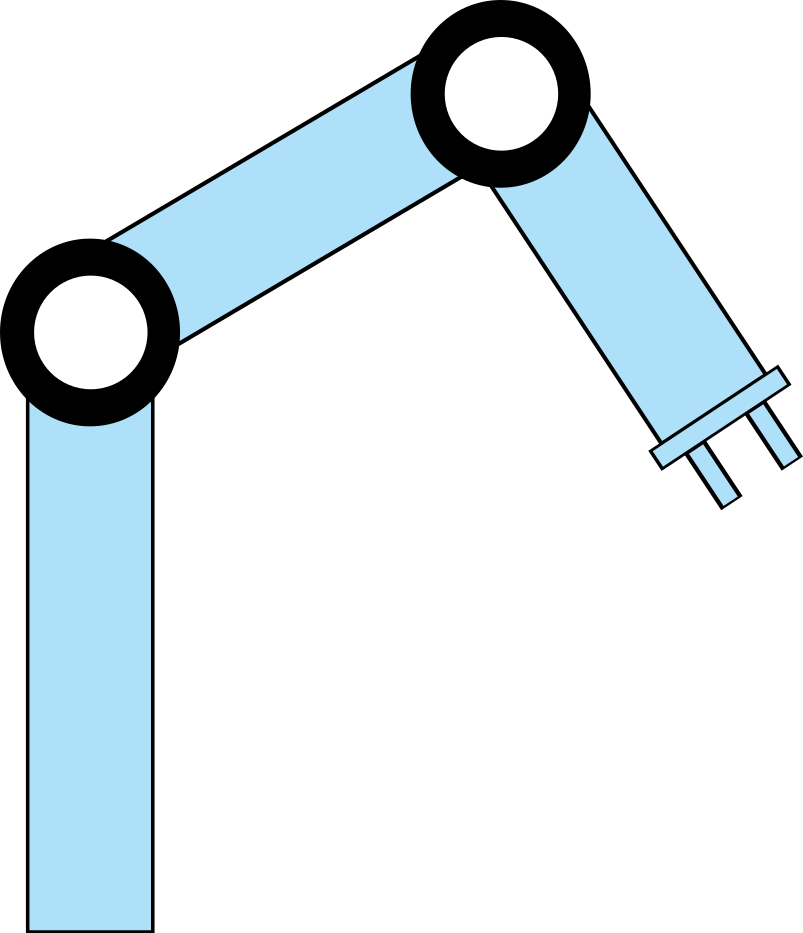
\includegraphics[width=0.35\textwidth]{imagenes/brazo-propio}
    \caption{Cadena cinemática abierta simple.}
    \label{fig:brazo-propio}
\end{figure}


\begin{itemize}
    \item Primero definimos el \textbf{marco de referencia} del mundo $(x_w, y_w, z_w)$, la letra $w$ viene de \textit{world}. El eje $y_w$ se alinea con el eslabón base (el primer eslabón) apuntando hacia el primer nodo, y el origen lo ubicamos en el inicio del eslabón base. Lo ejes $x_w$ y $z_w$ se colocan siguiendo el sistema de la mano derecha. En la figura~\ref{fig:brazo-marco-mundo} podemos ver cómo se coloca este marco.
    \begin{figure}[H]
        \centering
        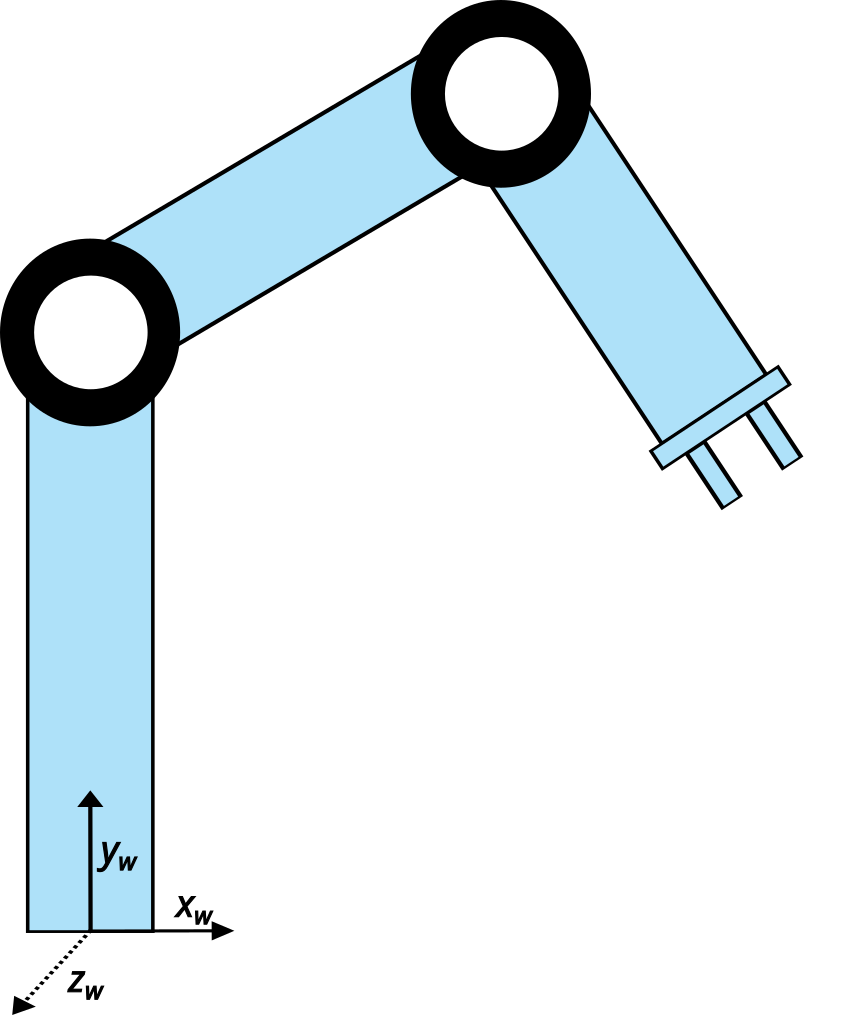
\includegraphics[width=0.35\textwidth]{imagenes/brazo-marco-mundo.png}
        \caption{Marco del mundo en cadena cinemática.}
        \label{fig:brazo-marco-mundo}
    \end{figure}
    \item Ahora procederemos a asignar un marco de referencia al primer nodo. Alineamos el eje $z_0$ con el eje en movimiento de la primera articulación. Luego alineamos el eje $x_0$ con el eslabón base, de forma que $x_0$ apunte hacia adentro del eslabón. Luego colocamos el eje $y_0$ siguiendo el sistema de la mano derecha. En la figura~\ref{fig:brazo-marco-primer-art} podemos ver cómo se asigna este marco de referencia. 
    \begin{figure}[H]
        \centering
        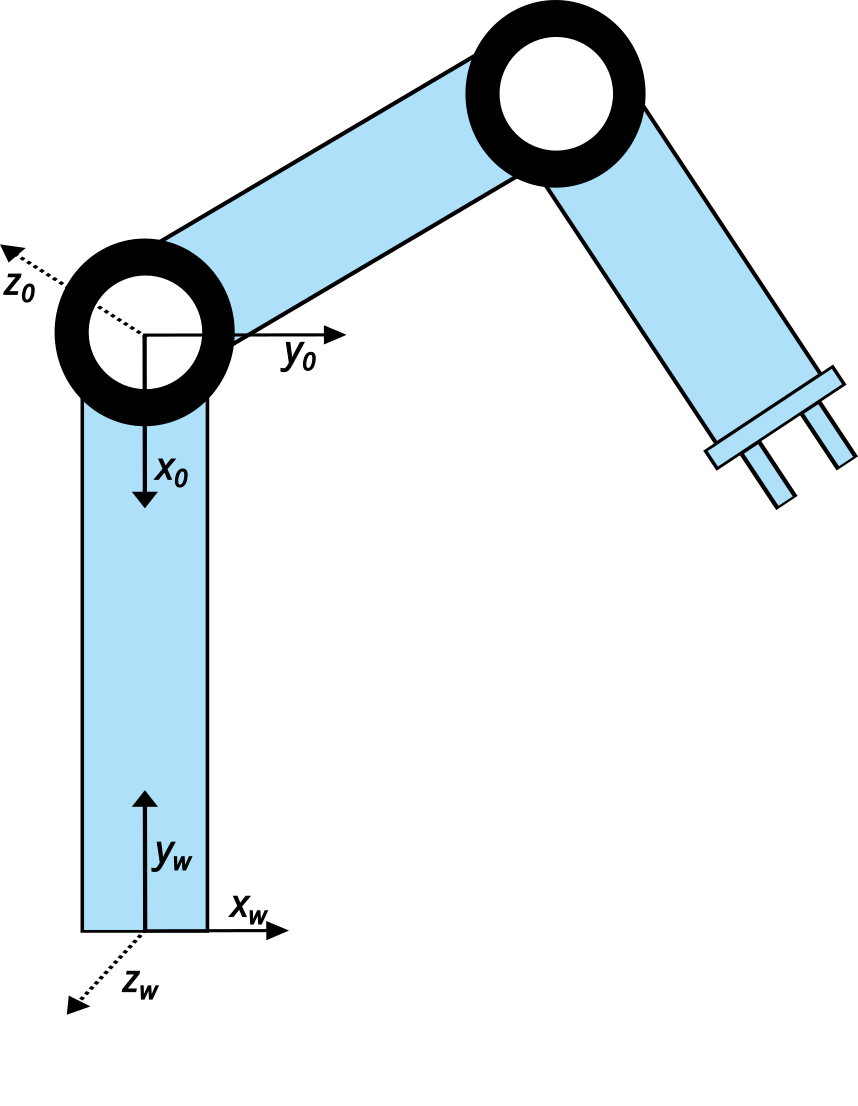
\includegraphics[width=0.35\textwidth]{imagenes/brazo-marco-primer-art}
        \caption{Marco del primer nodo.}
        \label{fig:brazo-marco-primer-art}
    \end{figure}
    \item Ahora procederemos a usar el método D-H que definimos anteriormente, pues lo definimos para eslabones con dos articulaciones. Respecto al eslabón $1$ (en este caso $i=1$), alineamos el eje $z_1$ con el eje en movimiento de la articulación distal. Alineamos el eje $z_0$ con el eje en movimiento de la articulación proximal. La articulación distal tendrá índice $2$, y la articulación proximal tendrá índice $1$. El origen $o$ del marco de referencia se coloca en la intersección entre el eje $z_1$ y el vector normal común a los ejes $z_1$ y $z_0$. El eje $x_1$ va de $z_0$ y $z_1$. El eje $y_1$ se elige con la regla de la mano derecha. La figura~\ref{fig:brazo-marco-dh} muestra cómo queda colocado este marco de referencia. 
    \begin{figure}[H]
        \centering
        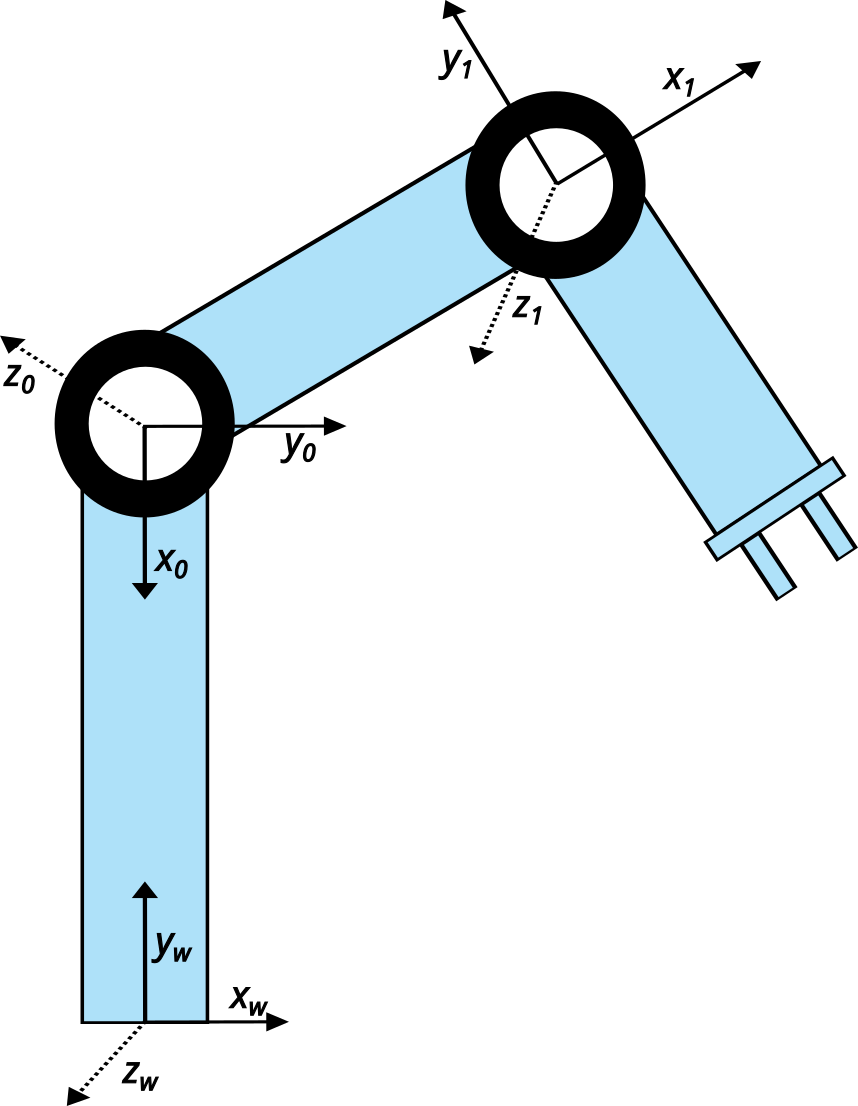
\includegraphics[width=0.35\textwidth]{imagenes/brazo-marco-dh.png}
        \caption{Marco del segundo nodo.}
        \label{fig:brazo-marco-dh}
    \end{figure}
    \item Y con eso terminamos de asinar los marcos de referencia a la cadena cinemática de la figura~\ref{fig:brazo-propio} con dos articulaciones. 
\end{itemize}
\section{Matrices de Transformación}
\subsection{Transformaciones}
Una transformación en D-H es una matriz que nos sirve para ubicar a un marco de referencia respecto de otro. Por tanto, también nos sirve para ubicar a un punto dentro de un marco de referencia desde la perspectiva de otro marco de referencia sin mover a dicho punto en el espacio. 

Para poder ubicar a un marco $i$ de referencia respecto de otro marco $j$, vamos a rotar (girar) y trasladar al marco $i$ hasta que se sobreponga al marco $j$. 

Veamos un ejemplo. En la figura~\ref{fig:transformacion-ejes} tenemos a un marco de referencia $i$ (los subíndices de sus ejes son $i$) en un plano $P_i$, también tenemos un marco de referencia $i-1$ en un plano $P_{i-1}$. Vamos a sobreponer el marco $i$ sobre el $i-1$. Notemos que el marco de referencia $i$ es el que se ubica sobre la articulación $i+1$ de una cadena cinemática, y el marco $i-1$ es el que se coloca sobre la articulación $i$ de la misma cadena, por tanto, el eslabón que une a estos marcos de referencia es el eslabón $i$.

\begin{figure}[H]
        \centering
        \includegraphics[width=0.35\textwidth]{imagenes/transformacion-ejes.png}
        \caption{Dos marcos de referencia.}
        \label{fig:transformacion-ejes}
\end{figure}

Primero, D-H nos indica que rotemos el marco $i$ alrededor del eje $x_i$ para alinear el eje $z_i$ con el eje $z_{i-1}$. Definimos $\beta_i$ como el ángulo de rotación alrededor del eje $x_i$. El marco $i$ rotado lo definiremos como marco $i'$ como se muestra en la figura~\ref{fig:prueba1}.

\begin{figure}[H]
        \centering
        \includegraphics[width=0.35\textwidth]{example-image-a}
        \caption{.}
        \label{fig:prueba1}
\end{figure}

Luego, realizaremos una traslación a lo largo del eje $x_i$ para pasar del plano $P_i$ al plano $P_{i-1}$, es decir, colocaremos los origenes sobre el mismo plano. A esta translación o desplazamiento lineal la definiremos como $b_i$. Procedemos a definir al marco $i$ rotado y trasladado como el marco $k$. Este paso se muestra en la figura~\ref{fig:prueba2}.

\begin{figure}[H]
        \centering
        \includegraphics[width=0.35\textwidth]{example-image-a}
        \caption{.}
        \label{fig:prueba2}
\end{figure}

Después, rotaremos el marco $k$ sobre el eje $z_{i-1}$ (que coincide con el eje $z_k$) para alinear los ejes $x$ y $y$. A esta rotación la definimos como $\theta_i$, además, esta rotación es justo la que realizó la articulación revoluta $i$ (la articulación $i$ es la del marco $i-1$). Si la articulación $i$ no es revoluta, entonces $\theta_i$ es cero. Entonces, si la articulación $i$ es revoluta, $\theta_i$ es la \textbf{variable de articulación}. Al marco $k$ rotado lo llamaremos $k'$. La figura~\ref{fig:prueba3} ilustra esta rotación.

\begin{figure}[H]
        \centering
        \includegraphics[width=0.35\textwidth]{example-image-a}
        \caption{.}
        \label{fig:prueba3}
\end{figure}
 
Por último, se realiza una traslación del marco $k'$ sobre el eje $z_{i-1}$. Y el marco $k'$ trasladado ya se sobrepone perfectamente al marco $i-1$. El marco $k'$ trasladado es el marco $i-1$ como se ve en la figura~\ref{fig:prueba4}. A esta traslación o desplazamiento lineal lo llamamos $d_i$, y si la articulación $i$ es prismática, entonces $d_i$ coincide con el desplazamiento de esta articulación, y además $d_i$ se le llama \textbf{variable de articulación}. Si la articulación $i$ no es prismática, entonces $d_i$ vale cero.

\begin{figure}[H]
        \centering
        \includegraphics[width=0.35\textwidth]{example-image-a}
        \caption{.}
        \label{fig:prueba4}
\end{figure}

Como se explicó anteriormente, D-H indica cómo colocar los marcos de referencia a una cadena cinemática abierta simple, e indica en qué orden ejecutar rotaciones y traslaciones para transformar un marco de referencia en otro. Claramente se puede lograr la transformacion con un diferente orden de rotaciones y traslaciones, pero D-H define esa convención de orden. 

\subsection{Parámetros D-H}
Los parámetros D-H son los que mencionamos anteriormente como $\beta_i$, $b_i$, $\theta_i$ y $d_i$.

\begin{miDefinicion}{Parámetros D-H}
    Para expresar las coordenadas del marco $i$ con respecto al marco $i-1$ sean:
    \begin{itemize}
        \item $\beta_i$: ángulo de rotación alrededor del eje $x_i$ para alinear los ejes $z$.
        \item $b_i$: desplazamiento lineal a lo largo del eje $x_i$ para colocar los orígenes sobre el mismo plano. 
        \item $\theta_i$: ángulo de rotación alrededor del eje $z_{i-1}$, que es la \textit{variable de la articulación} si $i$ es una articulación revoluta. 
        \item $d_i$: desplazamiento lineal a lo largo del eje $z_{i-1}$, que es la \textit{variable de la articulación} si la articulación $i$ es prismática. 
    \end{itemize}
\end{miDefinicion}

\subsection{Matriz de Transformación Homogénea}
Una transformación es una matriz que permite expresar las coordenadas de un marco respecto de otro marco. A esta matriz la llamamos \textbf{matriz de transformación homogénea}.

\begin{miDefinicion}{Matriz de Transformación Homogénea}
    Una matriz de transformacion homogénea ${}^jM_i$ es es una matriz de $4x4$ que permite expresar las coordenadas de un marco de referencia $i$ respecto del marco de referencia $j$ (sobrepone el marco $i$ sobre el $j$). 

    La estructura de una matriz de transformación homogénea es la siguiente:

    \begin{equation*}
        {}^jM_i = \begin{pmatrix}
                    R_{3x3} & P_{3x1} \\
                    F_{1x3} & W_{1x1} 
                    \end{pmatrix}
    \end{equation*}

    donde $R_{3x3}$ son las entradas que describen rotación, $P_{3x1}$ son las entradas que describen traslación, $F_{1x3}$ son entradas que describen perspectiva (siempre valen cero en D-H), y $W_{1x1}$ es la entrada que describe escalado (siempre vale 1 en D-H). 
\end{miDefinicion}

Utilizando el ejemplo anterior, utilizando los parámetros $\beta_i$, $b_i$, $\theta_i$ y $d_i$, la \textbf{matriz de transformacion homogénea} ${}^kM_i$ (la que transformará el marco $i$ en el marco $k$) se define como sigue:

\begin{equation}
    {}^kM_i = \begin{pmatrix}
                    1 & 0 & 0 & b_i \\
                    0 & \cos(\beta_i) & -\sin(\beta_i) & 0 \\
                    0 & \sin(\beta_i) & \cos(\beta_i) & 0 \\
                    0 & 0 & 0 & 1 
                    \end{pmatrix}
\end{equation}

La matriz anterior es la que realiza la rotación y la traslación sobre el eje $x_i$. 

La \textbf{matriz de transformacion homogénea} ${}^{i-1}M_k$ es la que realiza la rotación y la traslación sobre el eje $z_{i-1}$, y se define como sigue:

\begin{equation}
    {}^{i-1}M_k = \begin{pmatrix}
                    \cos(\theta_i) & -\sin(\theta_i) & 0 & 0 \\
                    \sin(\theta_i) & \cos(\theta_i) & 0 & 0 \\
                    0 & 0 & 1 & d_i \\
                    0 & 0 & 0 & 1 
                    \end{pmatrix}
\end{equation}

Por lo tanto, la \textbf{matriz de transformacion homogénea} ${}^{i-1}M_i$ es la siguiente multiplicación de matrices:

\begin{equation}
    {}^{i-1}M_i = {}^{i-1}M_k\times{}^kM_i
\end{equation}

A ${}^{i-1}M_i$ también la podemos definir de la siguiente forma, mostrando explícitamente todas las operaciones de rotación y traslación con sus respectivos parámetros que conlleva:

\begin{equation}
    {}^{i-1}M_i = Tra_{z_{i-1}}(d_i) Rot_{z_{i-1}}(\theta_i) Tra_{x_{i}}(b_i) Rot_{x_{i}}(\beta_i)
\end{equation}

\todo[inline]{Aquí voy a poner qué es una transformación (el interpretar un marco respecto de otro). Voy a poner cómo se ve (lo que se ve en la diapositiva 10 de la presentación D-H), los parámetros D-H, y finalmente cómo se insertan los parámetros en la matriz de transformación, finalmente un ejemplo rápido. Puedo poder eso en otras subsecciones. También debería de poner qué es la cinemática directa e inversa y cómo se relaciona la directa con D-H (angulos de articulaciones-matrices de transformacion-cjto de todas las matrices de transformación son la cinemática directa-transformacion de un punto a otro sistema de coordenadas).}
 \section{Asignación Clásica y Alternativa}
 Hasta ahora hemos visto la \textbf{conveción clásica de D-H} para asignar los índices de marcos de referencia y parámetros a una cadena cinemática abierta simple. Sin embargo, también existe la \textbf{conveción modificada de D-H} que utilizan libros como \textit{Introducción a la Robótica: Mecánica y Control (3.ª edición)}[4]. Cabe destacar que el conteo (primer, segundo, ...) e indexado (0, 1, ...) de los eslabones y articulaciones es igual en ambas conveciones.

 \subsection{Convención clásica D-H}
Se asignan los marcos de referencia y los parámetros como lo hemos visto hasta ahora. Es decir, el índice $i$ de un eslabón $l_i$ se utiliza para los índices del sistema de coordenadas de la articulación $i+1$. Se dice que los parámetros de esta conveción clásica son \textbf{parámetros distales}. En la figura~\ref{fig:convencion-clasica} se muestra esta convencion clásica.

\begin{figure}[H]
        \centering
        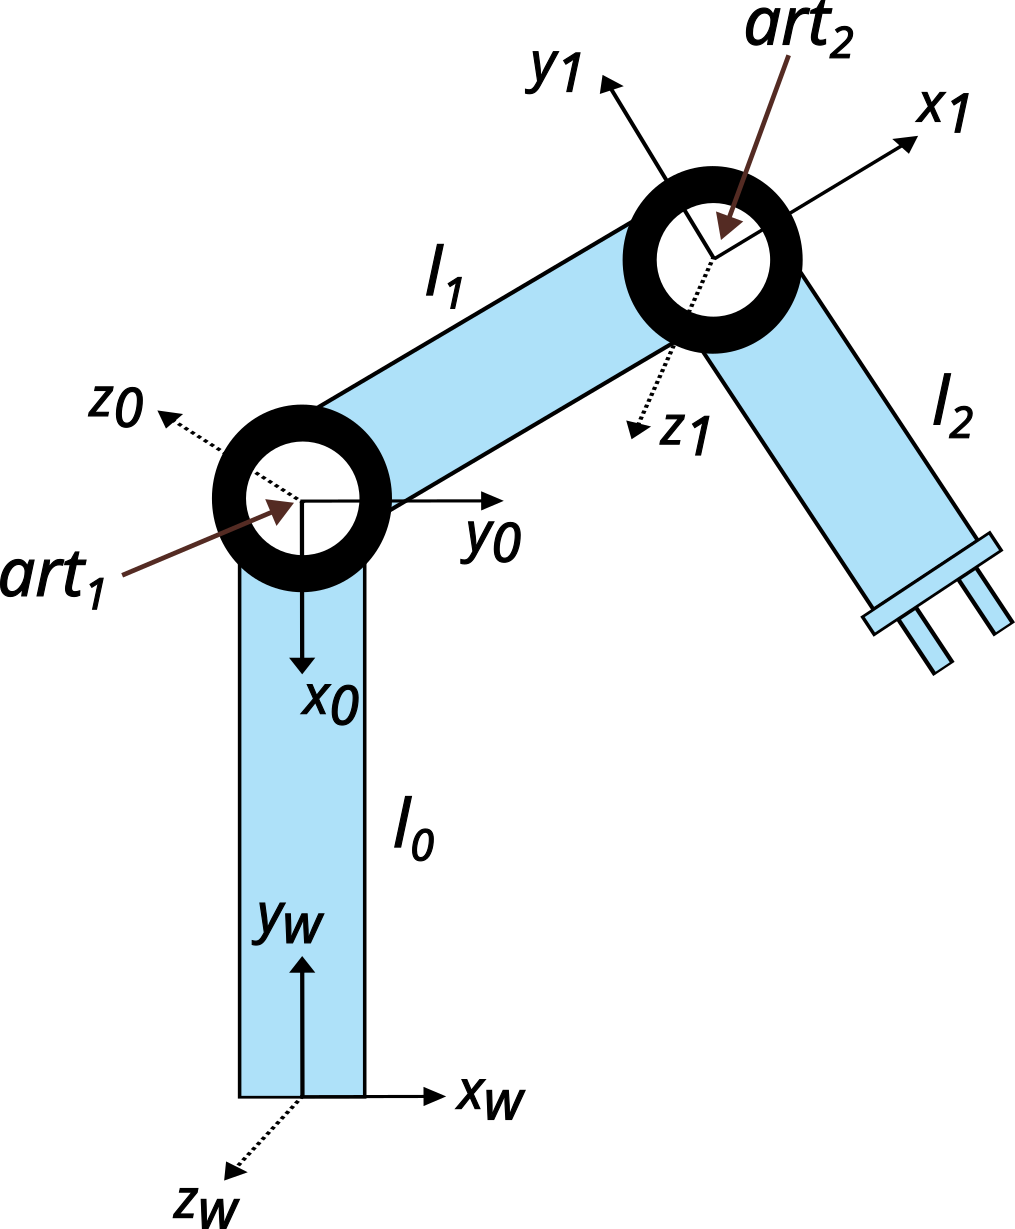
\includegraphics[width=0.45\textwidth]{imagenes/convencion-clasica.png}
        \caption{Convención clásica D-H.}
        \label{fig:convencion-clasica}
\end{figure}

 \subsection{Convención modificada o alternativa D-H}
 En esta convención, el índice $i$ de un eslabón $l_i$ se utiliza para los índices del sistema de coordenadas de la articulación $i$. Se dice que los parámetros de este convención modificada son \textbf{parámetros proximales}. En la figura~\ref{fig:convencion-modificada} se muestra esta convencion modificada.

 \begin{figure}[H]
        \centering
        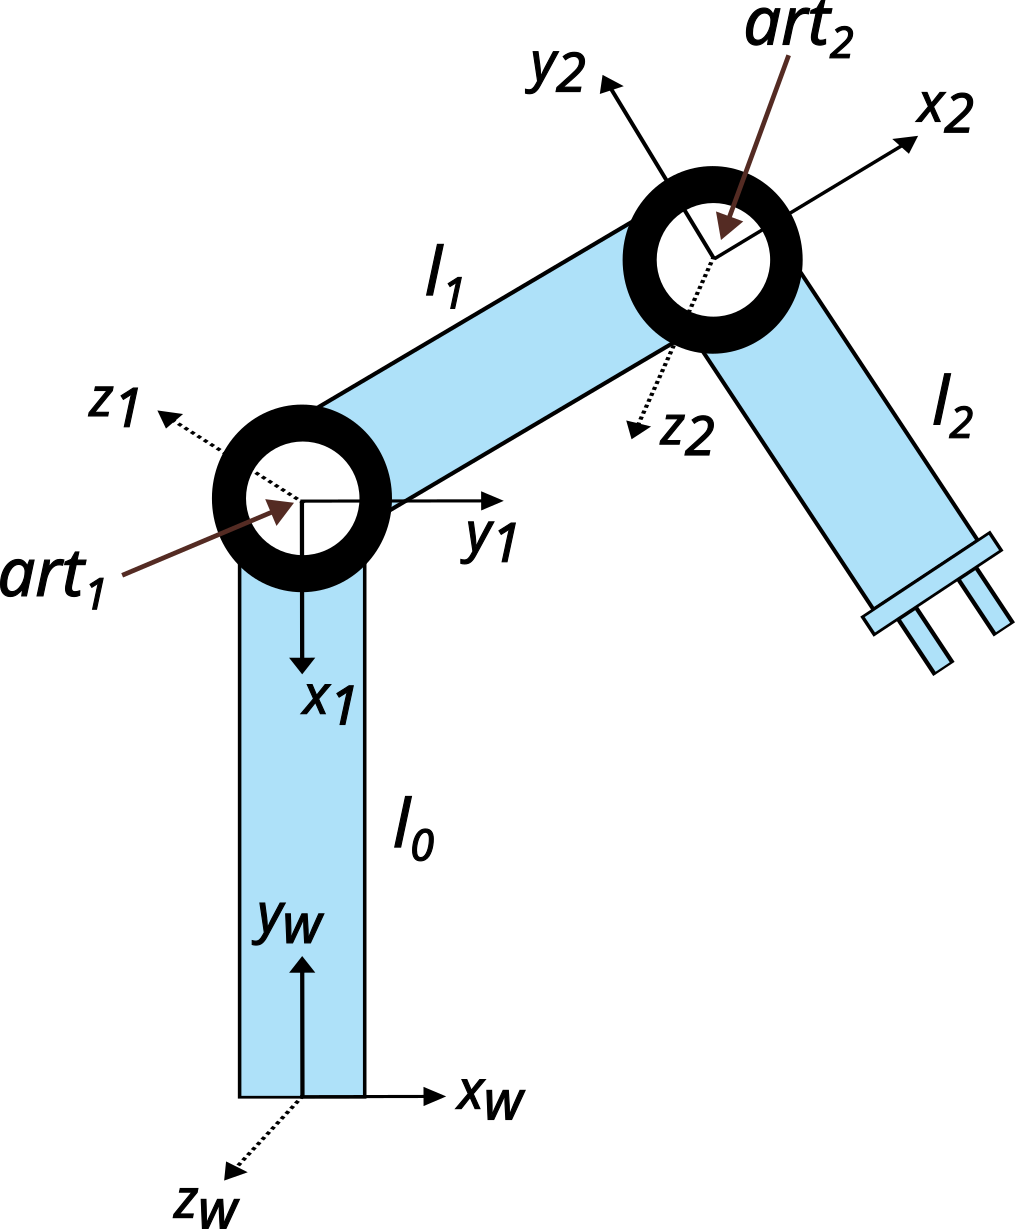
\includegraphics[width=0.45\textwidth]{imagenes/convencion-modificada.png}
        \caption{Convención modificada D-H.}
        \label{fig:convencion-modificada}
\end{figure}



\section{Cinemática directa e inversa}
La \textbf{cinemática} de un robot estudia el movimiento de sus partes sin considerar las fuerzas que lo producen. 

Para una \textbf{cadena cinemática abierta simple}, la \textbf{cinemática directa} calcula la posición y orientación del efector final respecto del \textbf{marco de referencia del mundo} a partir de los ángulos o movimientos de sus articulaciones. La \textbf{cinemática inversa} hace lo contrario, calcula qué valores deben tener los ángulos o movimientos de las articulaciones para que el efector final llegue a un punto deseado respecto del \textbf{marco de referencia del mundo}. \todo[inline]{basado de una visión general de IA de google con el prompt -cinemática directa e inversa de un robot-}

El método D-H es necesario para, de entre otras cosas, resolver el problema de la cinemática directa. El flujo para resolver el problema de la cinemática directa es este:
\begin{enumerate}
    \item Tomar los ángulos o desplazamientos de las articulaciones
    \item Construir todas las matrices de transformación
    \item Ubicar el efector final 
\end{enumerate}
%\section{Cinemática Inversa}
\todo[inline]{Poner lo de la última diapositiva}
\section{Datos Extras}
\subsection{Articiones prismáticas en D-H}
En este artículo consideramos que entre el eslabón base y el efector final sólo existen articulaciones revolutas, sin embargo el método D-H también cubre el caso cuando existe justamente una articulación prismática entre el eslabón base y el efector final. Tal articulación prismática se considera como un nodo en la cadena cinemática, y la forma en la que se le asigna un marco de referencia es diferente. Puedes investigar más sobre eso. [me lo dijo Gemini y resúmenes de IA de google, y mi propio entendimiento del tema]
\subsection{¿Los marcos de referencia se asignan a los nodos o a los eslabones?}
Realmente los marcos de referencia se asignan a los eslabones y NO a los nodos. Aunque en los dibujos básicamente colocamos los marcos sobre los nodos, el objetivo de estos marcos es ubicar a los eslabones (y no a los nodos). Los eslabones son cuerpos que ocupan espacio en el mundo real, los nodos son sólo el eje de movimiento relativo entre dos cuerpos, son puntos en el espacio, son intangibles. Un marco de referencia sirve para indicarte dónde empieza un eslabón y/o dónde termina otro. Los marcos son para ubicar eslabones. Entonces lo correcto es decir que los marcos se asignan a los eslabones (y no a los nodos). [me lo dijo Gemini]
\subsection{¿La pinza de un brazo robótico es un eslabón?}
Los eslabones son piezas sólidas que se conectan por articulaciones. Si una pinza de un brazo robótico empieza con un eslabón, entonces sí, la pinza es un eslabón porque es una pieza sólida que tiene una articulación que se conecta a otro eslabón. De hecho, esa pinza es el efector final (último eslabón) y además es la herramienta del efector final.

Sólo quiero mencionar que si después del último nodo (la articulación proximal de toda la cadena cinemática) tenemos un pedazo de tubo sólido largo y en el extremo de éste tenemos una piza (pero no hay otra articulación entre el pedazo de tubo y la pinza, sino que están empotrados), entonces el pedazo de tubo y la pinza son un sólo eslabón (el efector final). Aunque el tubo y la pinza son diferentes, dado que no hay una articulación entre ambos, entonces éstos juntos son el último eslabón (la pinza no es un eslabón diferente en sí misma). 
\subsection{Articulación prismática en pinza}
Respecto a la subsección anterior, si la pinza tiene una articulación prismática, ¿se le puede asignar un marco de referencia a la articulación prismática de la pinza (aunque no haya una articulación revoluta entre la pinza y el tubo)?

Usualmente la articulación prismática de una pinza de una brazo robótico no se considera como nodo en D-H, esto porque el objetivo de D-H es ubicar en el espacio al efector final de un brazo robótico, y para ello basta con ubicar el marco del tubo (que es como el chasis o cuerpo de la pinza). El abrir y cerrar de la pinza no cambia la posición de la herramienta (la pinza) en el espacio, sólo cambia su estado de agarre. La articulación prismática de la pinza se considera un mecanismo de actuación independiente. 

Sin embargo, si quisieras ubicar en el espacio una punta de la pinza, entonces sí se necesitaría asignar un marco de referencia a la articulación prismática de la pinza. Y el método de D-H funcionaría bien para ubicar una punta de la pinza (sería como reinterpretar al efector final como una punta de la pinza en lugar de toda la pinza). D-H no funcionaría para ubicar a las dos pinzas aunque se le asignara un marco a la articulación prismática porque entonces tendríamos dos efectores finales, es decir, tendríamos una cadena cinemática abierta no simple (ya no sería una secuencia lineal de eslabones, sino un árbol). Bueno, ahora que lo pienso, podríamos ejecutar D-H dos veces, una para cada dedo de la pinza. 
\section{Referencias}
[2] \url{https://en.wikipedia.org/wiki/Frame_of_reference}

[3] El resumen de IA de google con el prompt -cadena cinemática abierta simple robotica-.

[4] \url{https://en.wikipedia.org/wiki/Denavit%E2%80%93Hartenberg_parameters}

% Fin del documento
\end{document}
